\documentclass[12pt]{article}
\usepackage[all, stdclass]{lix}
\usepackage{graphicx}
\usepackage{svg}
\usepackage{circuitikz}
\usepackage{amsmath}
\usepackage{bookmark}
\usepackage{gensymb}
\svgsetup{
  inkscapepath=assets/,  % Path to the directory containing your SVG files
  svgpath=assets/        % Path to the directory containing your SVG files
}
\usepackage{float}
\usepackage{hyperref}
% \usepackage{graphicx}
\usepackage{times}


%----------EDIT COVER INFO HERE -----------------%

\def \LOGOPATH {assets/birzeit-logo.png}
\def \DEPARTEMENT {Department of Electrical \& Computer Engineering}
\def \COURSENUM {ENEE2103}
\def \COURSENAME {Circuits and Electronics Laboratory}
\def \REPORTTITLE {Filters}
\def \STUDENTNAME {Mohammad Abu-Shelbaia}
\def \PARTNERAN {Nidal Zabade}
\def \PARTNERBN {Mahmoud Shihab}
\def \PARTNERAID {1200153}
\def \PARTNERBID {1182143}
\def \STUDENTID {1200198}
\def \INSTRUCTOR {Dr. Mahran Quran }
\def \ASSISTANT {Eng. Raffah Rahal}
\def \REPORTNUM {5}

%--------------------BORDERS----------------------------%
% \usepackage{parskip}
% \setlength{\parskip}{0pt}
% \geometry{top=1.54cm}
% \usepackage{everyshi}
% \usepackage{tikz}
% \EveryShipout{%
%     \begin{tikzpicture}[overlay,remember picture]
%         \draw [line width=0.5pt]
%             ($ (current page.north west) + (1cm,-1cm) $)
%             rectangle
%             ($ (current page.south east) + (-1cm,1cm) $);
%     \end{tikzpicture}
% }
%------------------------------------------------%


\begin{document}

\begin{titlepage}
    \vfill
    \begin{center}
        \includegraphics[width=0.7\textwidth]{\LOGOPATH} \\
        \hfill \\
        \Large{\DEPARTEMENT} \\
        \Large{\COURSENUM\;-\;\COURSENAME} \\
        \vfill
        \textbf{\LARGE{Experiment \#\REPORTNUM}} \\
        \textbf{\LARGE{\REPORTTITLE}}
    \end{center}
    \vfill
    \begin{flushleft}
        \Large{\textbf{Prepared by:}\\ \STUDENTNAME\quad\STUDENTID} \\
        \Large{\textbf{Partners:}\\ 
        \begin{tabular}{@{}l@{\quad}l}
            \PARTNERAN & \PARTNERAID \\
            \PARTNERBN & \PARTNERBID \\
        \end{tabular}} \\
        \Large{\textbf{Instructor:} \INSTRUCTOR} \\
        \Large{\textbf{Assistant:} \ASSISTANT} \\
        \Large{\textbf{Section:} 4}\\
        \LARGE{\textbf{ }}\\
        \LARGE{\textbf{ }}\\
        \LARGE{\textbf{ }}\\
        \Large{\textbf{Date:} \today}\\
    \end{flushleft}
    \vfill
\end{titlepage}

\clearpage
% --------------- ABSTRACT ------------------%
% ---- TABLES --------------------------------%
{
\centering
\section*{Abstract}
In this experiment, we talk about filters, filter types: passive or active, filter order, cut-off frequency, 3db cut-off frequency, how to work practically with filters and the advantage of using an active filter, and the effect of frequency on the circuit. The tools required to carry out this experiment are DMM, oscilloscope, power-supply, function generator, an uA741 operation amplifier, resistors, capacitors, and an inductance decade box.
\clearpage
}
\tableofcontents
\clearpage
\setlength{\parskip}{\baselineskip}%
\listoffigures
\clearpage
\listoftables
\clearpage
\pagenumbering{arabic}
%-------------- CONTENT ---------------------%


\clearpage
\h{Theory}
Filters in circuits allow certain frequencies to pass through while blocking undesired frequencies. Filters are classified into two types: passive and active filters. Passive filters are made of passive components such as resistors, capacitors, and inductors. Active filters are made of active components such as transistors and op-amps. A filter order is the number of reactive components in the filter.
Furthermore, filters have four basic types: low pass, high pass, band pass, and band stop. 
\hh{Passive Filters}
\hhh{Low Pass Filter}
As the name suggests, this type of filter allows low frequencies to pass through while blocking high frequencies.
\begin{figure}[H]
    \centering
    \resizebox{0.40\textwidth}{!}{%
    \begin{circuitikz}
    \tikzstyle{every node}=[font=\LARGE]
    % \draw (-13,13) to[short, -*] (-13,13);
    \draw (-5,7) to[R] (-2.25,7);
    \draw (-2.25,7) to[C] (-2.25,4.75);
    \draw[] (-2.25,4.75) to[short] (-5,4.75);
    \draw [](-2.5,4.75) to[short] (-1,4.75);
    \draw [](-2.25,7) to[short] (-1,7);
    \draw [](-5,7) to[short, -o] (-5.25,7);
    \draw [](-5,4.75) to[short, -o] (-5.25,4.75);
    \draw [](-1,4.75) to[short, -o] (-0.75,4.75);
    \draw [](-1.25,7) to[short, -o] (-0.75,7);
    \node [font=\large] at (-5.25,5.875) {$V_i$};
    \node [font=\large] at (-0.5,5.875) {$V_o$};
    \end{circuitikz}
    }
    \resizebox{0.40\textwidth}{!}{%
    \begin{circuitikz}
    \tikzstyle{every node}=[font=\LARGE]
    % \draw (-13,13) to[short, -*] (-13,13);
    \draw (-5,7) to[L] (-2.25,7);
    \draw (-2.25,7) to[R] (-2.25,4.75);
    \draw[] (-2.25,4.75) to[short] (-5,4.75);
    \draw [](-2.5,4.75) to[short] (-1,4.75);
    \draw [](-2.25,7) to[short] (-1,7);
    \draw [](-5,7) to[short, -o] (-5.25,7);
    \draw [](-5,4.75) to[short, -o] (-5.25,4.75);
    \draw [](-1,4.75) to[short, -o] (-0.75,4.75);
    \draw [](-1.25,7) to[short, -o] (-0.75,7);
    \node [font=\large] at (-5.25,5.875) {$V_i$};
    \node [font=\large] at (-0.5,5.875) {$V_o$};
    \end{circuitikz}
    }
    \label{fig:Low-Pass}
    \caption{$1^{st}$ Order Passive Low-Pass filters}
\end{figure}
% \begin{equation} \label{eq1}
\begin{equation}
\begin{aligned}
            V_o &= \frac{X_c}{X_c + X_r} \times V_i  \quad\quad &V_o &= \frac{X_r}{X_r + X_l} \times V_i\\
            X_c &= \frac{1}{j\omega c}  &X_l &= j\omega l
\end{aligned}
\end{equation}
% \end{equation}
The frequency is inversely proportional to the impedance $X_c$, and $X_c$ is directly proportional to $V_o$, and by the same logic the frequency is directly proportional to $X_l$, and $X_l$ is inversely proportional to $V_o$, which indicates that higher frequencies generate low $V_o$ voltage (reject), and low frequencies generate high $V_o$ltage (pass).\\ \\
The cut-off frequency is the frequency at which a point of inversion occurs, which indicates what high and low frequencies are, and it's given by:
\begin{equation}
    \begin{aligned}
        f_c = \frac{1}{2\pi R C} \quad\quad or \quad\quad f_c = \frac{R}{2\pi L}
    \end{aligned}
\end{equation}
\hhh{High Pass Filter}
This type of filter is a complement of the low-pass filter since it rejects low frequencies and passes high ones.
\begin{figure}[H]
    \centering
    \resizebox{0.40\textwidth}{!}{%
    \begin{circuitikz}
    \tikzstyle{every node}=[font=\LARGE]
    % \draw (-13,13) to[short, -*] (-13,13);
    \draw (-5,7) to[C] (-2.25,7);
    \draw (-2.25,7) to[R] (-2.25,4.75);
    \draw[] (-2.25,4.75) to[short] (-5,4.75);
    \draw [](-2.5,4.75) to[short] (-1,4.75);
    \draw [](-2.25,7) to[short] (-1,7);
    \draw [](-5,7) to[short, -o] (-5.25,7);
    \draw [](-5,4.75) to[short, -o] (-5.25,4.75);
    \draw [](-1,4.75) to[short, -o] (-0.75,4.75);
    \draw [](-1.25,7) to[short, -o] (-0.75,7);
    \node [font=\large] at (-5.25,5.875) {$V_i$};
    \node [font=\large] at (-0.5,5.875) {$V_o$};
    \end{circuitikz}
    }
    \resizebox{0.40\textwidth}{!}{%
    \begin{circuitikz}
    \tikzstyle{every node}=[font=\LARGE]
    % \draw (-13,13) to[short, -*] (-13,13);
    \draw (-5,7) to[R] (-2.25,7);
    \draw (-2.25,7) to[L] (-2.25,4.75);
    \draw[] (-2.25,4.75) to[short] (-5,4.75);
    \draw [](-2.5,4.75) to[short] (-1,4.75);
    \draw [](-2.25,7) to[short] (-1,7);
    \draw [](-5,7) to[short, -o] (-5.25,7);
    \draw [](-5,4.75) to[short, -o] (-5.25,4.75);
    \draw [](-1,4.75) to[short, -o] (-0.75,4.75);
    \draw [](-1.25,7) to[short, -o] (-0.75,7);
    \node [font=\large] at (-5.25,5.875) {$V_i$};
    \node [font=\large] at (-0.5,5.875) {$V_o$};
    \end{circuitikz}
    }
    \label{fig:High-Pass}
    \caption{$1^{st}$ Order Passive High-Pass filters}
\end{figure}
\begin{equation}
    \begin{aligned}
                V_o &= \frac{X_r}{X_c + X_r} \times V_i  \quad\quad &V_o &= \frac{X_l}{X_r + X_l} \times V_i\\
                X_c &= \frac{1}{j\omega c}  &X_l &= j\omega l
    \end{aligned}
\end{equation}
According to the above equations, the frequency is inversely proportional to the impedance $X_c$, $X_c$ is inversely proportional to $V_o$, and by the same logic the frequency is directly proportional to $X_l$, and $X_l$ is directly proportional to $V_o$, which indicates that higher frequencies generate high $V_o$ltage (pass), and low frequencies generate low $V_o$ volltage (reject).\\ \\
The cut-off frequency is the frequency at which a point of inversion occurs, which indicates what high and low frequencies are, and it's given by:
\begin{equation}
    \begin{aligned}
        f_c = \frac{1}{2\pi R C} \quad\quad or \quad\quad f_c = \frac{R}{2\pi L}
    \end{aligned}
\end{equation}
\hhh{Band Pass Filter}
A band pass filter is a combination of a low pass and a high pass filter, which allows a certain band of frequencies to pass through while blocking the rest. It has two cut-off frequencies, $f_{c1}$ and $f_{c2}$, which are the frequencies at which the filter starts to reject frequencies. The bandwidth is the difference between the two cut-off frequencies. It is a second-order filter, which means that it has two reactive components.
\begin{figure}[H]
    \centering
    \begin{circuitikz}
    \tikzstyle{every node}=[font=\LARGE]
    % \draw (-13,13) to[short, -*] (-13,13);
    \draw(-7,7) to[L] (-5,7);
    \draw (-5,7) to[C] (-2.25,7);
    \draw (-2.25,7) to[R] (-2.25,4.75);
    \draw[] (-2.25,4.75) to[short] (-7,4.75);
    \draw [](-2.5,4.75) to[short] (-1,4.75);
    \draw [](-2.25,7) to[short] (-1,7);
    \draw [](-7,7) to[short, -o] (-7.25,7);
    \draw [](-7,4.75) to[short, -o] (-7.25,4.75);
    \draw [](-1,4.75) to[short, -o] (-0.75,4.75);
    \draw [](-1.25,7) to[short, -o] (-0.75,7);
    \node [font=\large] at (-7.25,5.875) {$V_i$};
    \node [font=\large] at (-0.5,5.875) {$V_o$};
    \end{circuitikz}
    \caption{$2^{nd}$ Order Passive Band-Pass filters}
\end{figure}
The center frequency and the cut-off frequencies are given by:
\math{_}{
    f_0 = {1 \over {2\Pi \sqrt{LC}}}
}
\math{_} {
    f_{c1} = {-{R \over 2L} + \sqrt{{R \over 2L}^{2} + {1 \over LC}} \over 2\Pi}
}
\math{_} {
    f_{c2} = {{R \over 2L} + \sqrt{{R \over 2L}^{2} + {1 \over LC}} \over 2\Pi}
}
\hh{Active Filters}
Passive RC filters such as low pass, high pass, and band pass filters use resistors and capacitors to filter electronic signals. However, the output signal is less than the input signal, which means that the signal gain is never greater than unity and load impedance affects the filter characteristics. Multi-stage passive filters can cause severe attenuation of the output signal. To control the loss of signal, active filters use active components such as transistors, FETs (Field Effect Transistors), and operational amplifiers in their design. These filters draw external power from the source to boost the output signal.\cite{ee-hub}
\begin{figure}[H]
    \centering
    \begin{circuitikz}
        \ctikzset{bipoles/length=1cm}
        \draw
        (0, 0) node[op amp] (opamp) {}
        (opamp.-) to[R,l_=$R_1$,-o] (-3, 0.35) 
        (opamp.-) to[short,*-] ++(0,0.5) coordinate (leftC)
        to[R=$R_2$] (leftC -| opamp.out)
        (opamp.-) to[short,*-] ++(0,1.5) coordinate (leftC) to[C=$C_1$] (leftC -| opamp.out) 
        to[short,-*] (opamp.out) to [short,-o] (1.5,0) 
        (opamp.+) -- (-1,-0.35) to (-1,-0.75) node[ground]{}
        ;
    \end{circuitikz}
    \caption{Active Low-Pass Filter}
\end{figure}
\clearpage
\h{Procedure and Data Analysis}
\hh{Passive Filters}
\hhh{First Order Filter}
\begin{figure}[H]
    \centering
    \begin{circuitikz}
        \tikzstyle{every node}=[font=\LARGE]
        % \draw (-13,13) to[short, -*] (-13,13);
        \draw (-5,7) to[C] (-2.25,7);
        \draw (-2.25,7) to[R] (-2.25,4.75);
        \draw[] (-2.25,4.75) to[short] (-5,4.75);
        \draw [](-2.5,4.75) to[short] (-1,4.75);
        \draw [](-2.25,7) to[short] (-1,7);
        \draw [](-5,7) to[short, -o] (-5.25,7);
        \draw [](-5,4.75) to[short, -o] (-5.25,4.75);
        \draw [](-1,4.75) to[short, -o] (-0.75,4.75);
        \draw [](-1.25,7) to[short, -o] (-0.75,7);
        \node [font=\large] at (-5.25,5.875) {$V_i$};
        \node [font=\small] at (-3.3, 5.875) {$2.2K\Omega$};
        \node[font=\small] at (-3.5, 8) {$220nF$};
        \node [font=\large] at (-0.5,5.875) {$V_o$};
    \end{circuitikz}
    \caption{1'st Order RC High-pass filter}
\end{figure}
The circuit above was connected, with a source $V_{i}$ that has 1V RMS Value, and a frequency of 20Hz. The cut-off frequency was found by setting the frequency that satisfies
\begin{equation}
    V_c = 0.706 \times V_{max}
\end{equation}
and it was found to be 318Hz it was also found that the phase shift between the input and output signal to be $44.7\ \degree$, as shown in the following figure:
\begin{figure}[H]
    \centering
    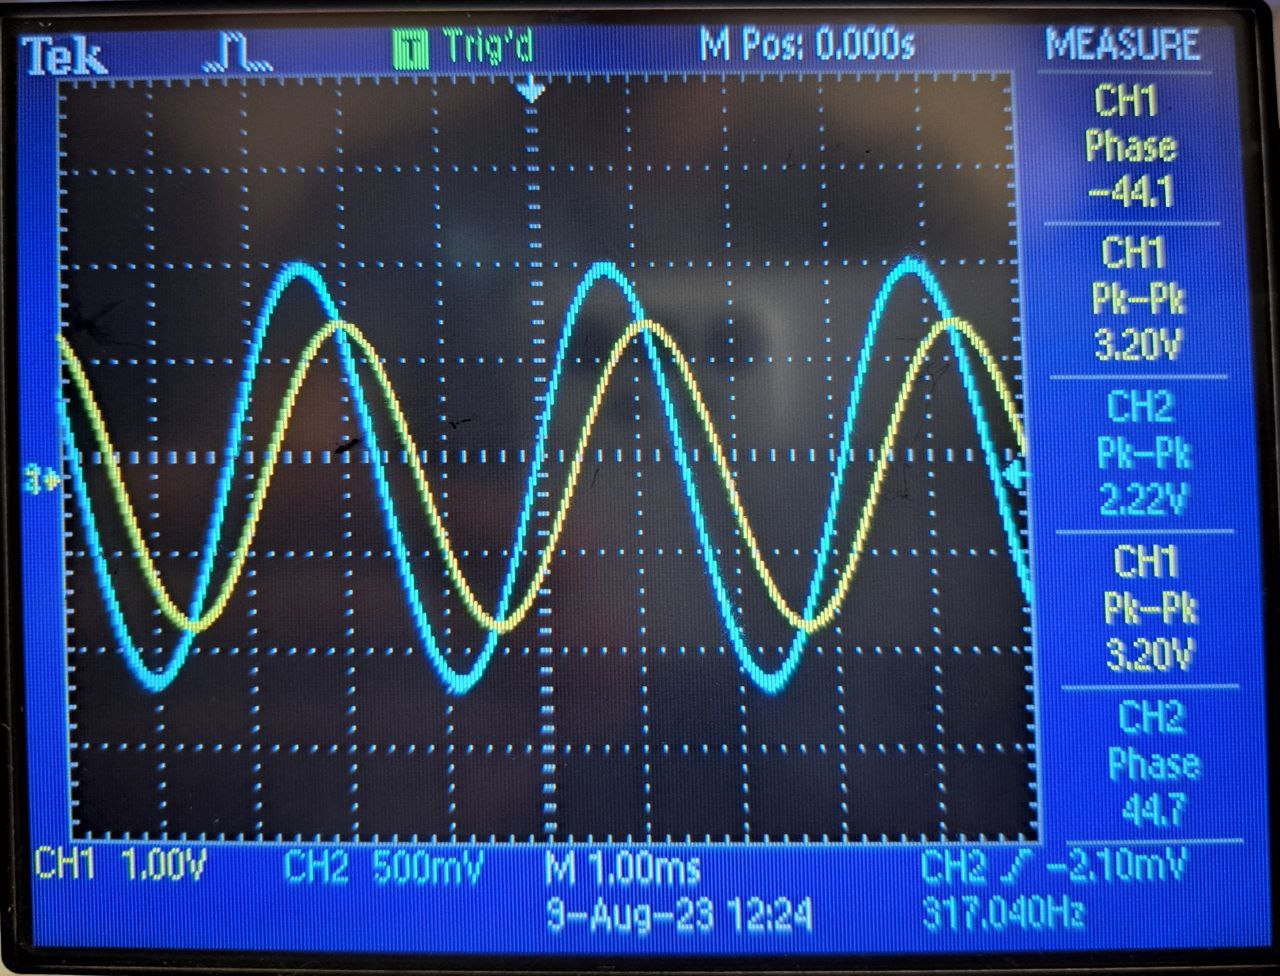
\includegraphics[width=0.5\textwidth]{assets/fc.jpg}
    \caption{Cut-off frequency and phase shift}
\end{figure}
% Please add the following required packages to your 
\begin{table}[H]
    \centering
    \resizebox{\textwidth}{!}{%
    \begin{tabular}{|c|c|c|c|c|c|}
    \hline
    Frequency (Hz) & Vin (Vrms) & Vc (Vrms) & Phase  & Log(f)      & 20Log(Vc/Vin) \\ \hline
    20             & 1          & 1.09      & -87.3  & 1.301029996 & 0.7485299588  \\ \hline
    31.8           & 1          & 1.08      & -92.3  & 1.50242712  & 0.6684751097  \\ \hline
    159            & 1          & 0.974     & -64    & 2.201397124 & -0.2288208624 \\ \hline
    318            & 1          & 0.774     & -45    & 2.50242712  & -2.225180786  \\ \hline
    636            & 1          & 0.487     & -26.9  & 2.803457116 & -6.249420776  \\ \hline
    1272           & 1          & 0.265     & -12.8  & 3.104487111 & -11.53508252  \\ \hline
    2544           & 1          & 0.135     & -6.45  & 3.405517107 & -17.39332463  \\ \hline
    3180           & 1          & 0.109     & -3.43  & 3.50242712  & -19.25147004  \\ \hline
    3816           & 1          & 0.091     & -3.01  & 3.581608366 & -20.81917215  \\ \hline
    4452           & 1          & 0.074     & -1.93  & 3.648555156 & -22.61536561  \\ \hline
    5088           & 1          & 0.07      & -1.83  & 3.706547103 & -23.0980392   \\ \hline
    6360           & 1          & 0.058     & -0.237 & 3.803457116 & -24.73144013  \\ \hline
    \end{tabular}%
    }
    \caption{Low-pass filter data points}
    \label{tab:my-table}
\end{table}
From the table above, $20\log{Vc\over Vin}$ was plotted against $log{f}$ using google sheets, from the plot we saw that it was a low-pass filter which indicated that the load on R is a high-pass filter, having the $-3dB$ point cross the x-axis at $\log{f} = 2.65$ hence, the 3dB cut-off frequency $f_{3dB} = 10^{2.75} = 562.34Hz$ which is not an accurate read and it goes back because there is no enough data point to the plot or an error rate in the DMM.
\begin{figure}[H]
    \centering
    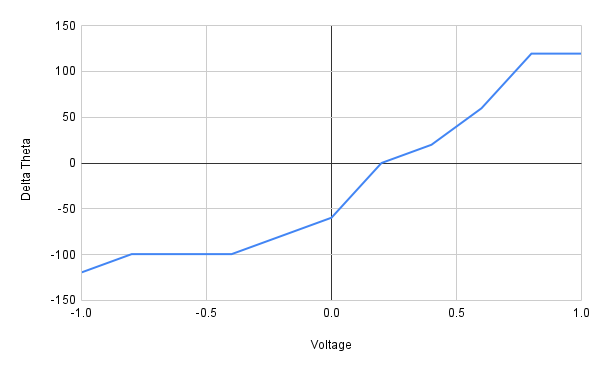
\includegraphics[width=0.7\textwidth]{assets/ch.png}
    \caption{$20\log{Vc\over Vin}$ vs $log{f}$}
    \label{meow-meow-n}
\end{figure}
\hhh{Second Order Filter}
\begin{figure}[H]
    \centering
    \begin{circuitikz}
    \tikzstyle{every node}=[font=\LARGE]
    % \draw (-13,13) to[short, -*] (-13,13);
    \draw(-7,7) to[L] (-5,7);
    \draw (-5,7) to[C] (-2.25,7);
    \draw (-2.25,7) to[R] (-2.25,4.75);
    \draw[] (-2.25,4.75) to[short] (-7,4.75);
    \draw [](-2.5,4.75) to[short] (-1,4.75);
    \draw [](-2.25,7) to[short] (-1,7);
    \draw [](-7,7) to[short, -o] (-7.25,7);
    \draw [](-7,4.75) to[short, -o] (-7.25,4.75);
    \draw [](-1,4.75) to[short, -o] (-0.75,4.75);
    \draw [](-1.25,7) to[short, -o] (-0.75,7);
    \node [font=\large] at (-7.25,5.875) {$V_i$};
    \node [font=\large] at (-0.5,5.875) {$V_o$};
    \node [font=\small] at (-3.5, 8) {$470 nF$};
    \node [font=\small] at (-6, 8) {$100 mH$};
    \node [font=\small] at (-1.5, 5.875) {$1 k\Omega$};
    \end{circuitikz}
    \caption{$2^{nd}$ Order RLC Band-Pass filters}
\end{figure}
The above circuit was connected to a 2V RMS power source with a frequency equal to the resonance frequency. theoretically, it's given by:
\math{_}{
    f_0 = {1 \over {2\pi \sqrt{LC}}} = 734.13Hz
}
and we got it experimentally by changing the frequency until the phase shift between $V_i$ and $V_o$ is equal to zero, which occurs at $f = 676.27 Hz$ as shown in the following figure:
\begin{figure}[H]
    \centering
    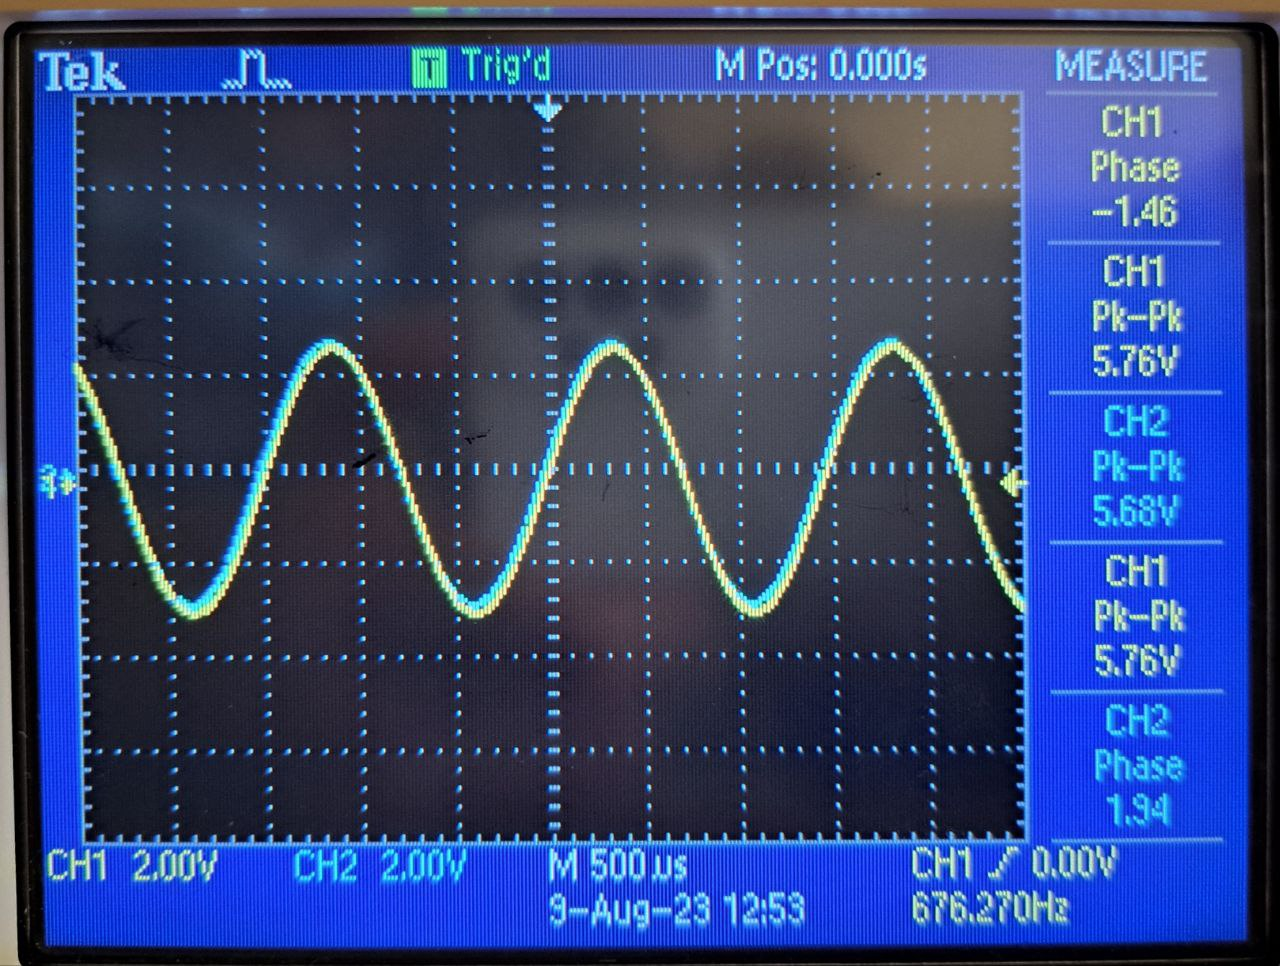
\includegraphics[width=0.5\textwidth]{assets/f0p2.jpg}
    \caption{Resonance[Center] Frequency of the band-pass filter}
\end{figure}
The method we used to find the cut-off frequency is by using the fact that at cut-off frequencies the maximum voltage drops to 0.707 of its value, hence it occurs at $Vc + Vl = 0.707 * 1.09 = 0.7707$ 2 times, one before the resonance frequency and the another after the resonance frequency as shown in the figure below:
\begin{figure}[H]
    \centering
    \resizebox{0.49\textwidth}{!}{
    \centering
    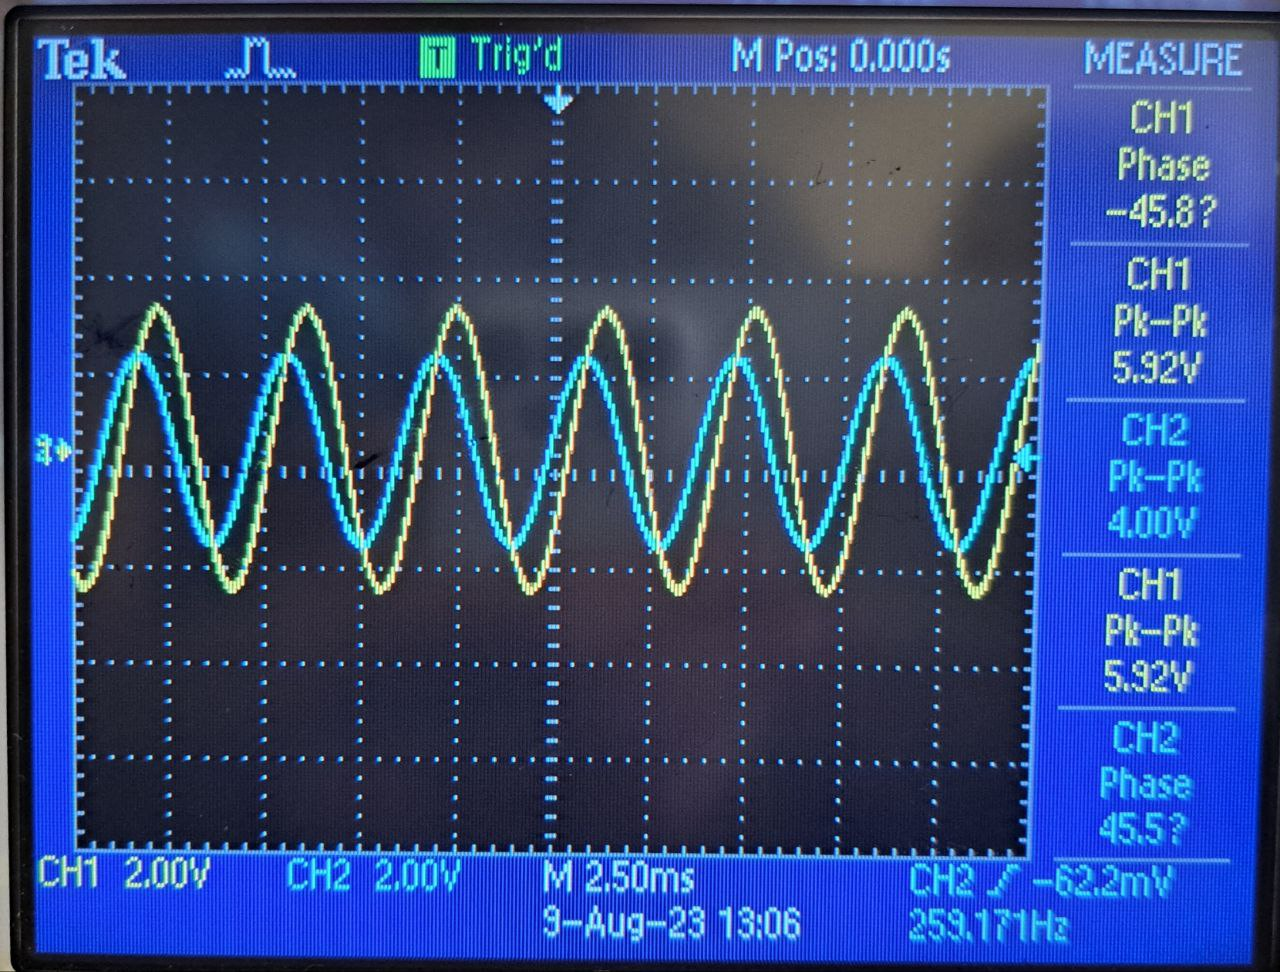
\includegraphics{assets/f01.jpg}
    }
    \resizebox{0.49\textwidth}{!}{
    \centering
    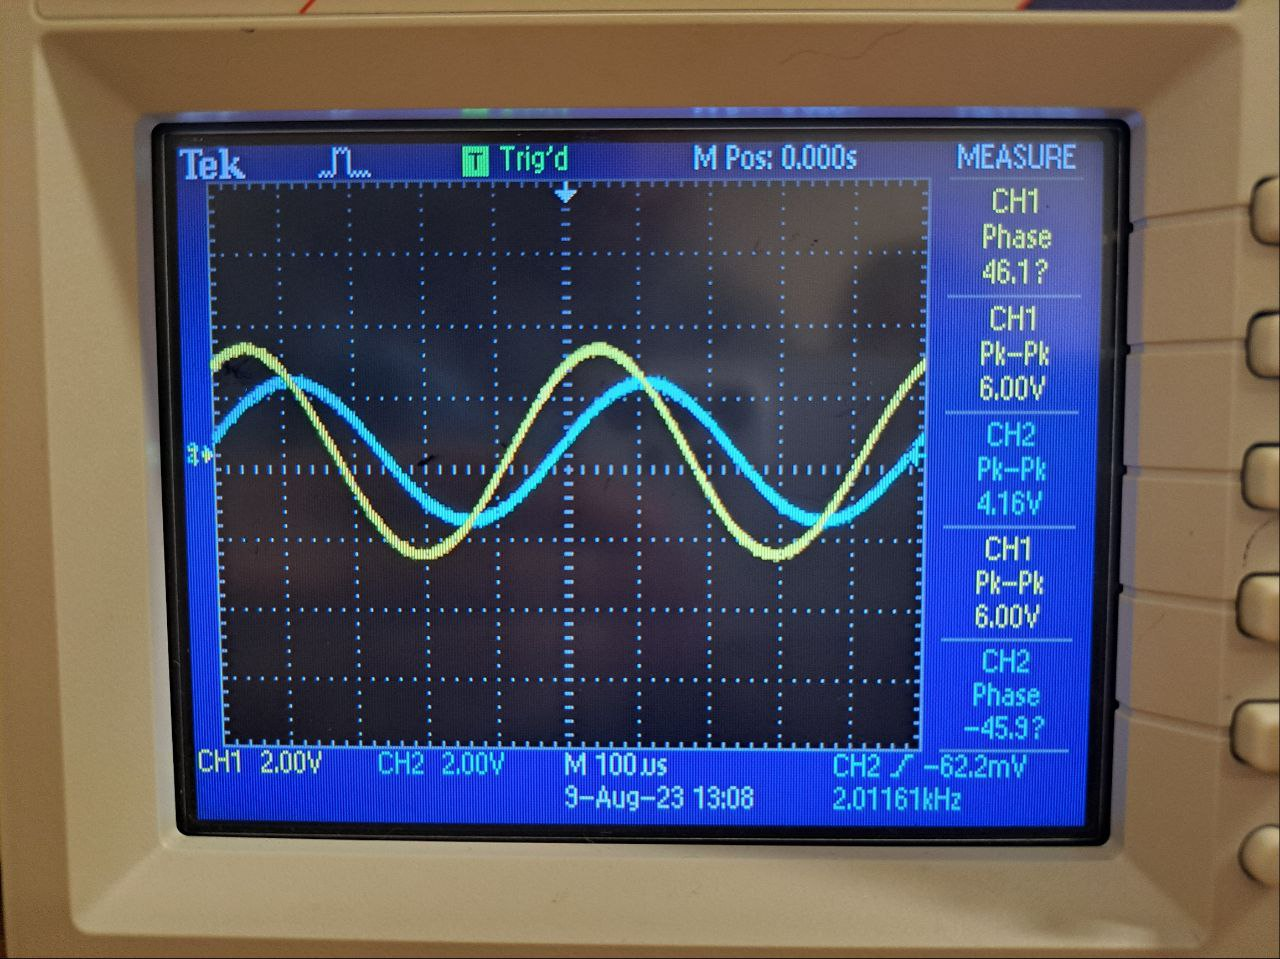
\includegraphics{assets/fc2.jpg}
    }  
    \caption{Band-pass filter cut-off frequencies}
\end{figure}
as shown above the two cut-off frequencies are 259.17Hz and 2016Hz.
% Please add the following required packages to your document preamble:
% \usepackage{graphicx}
% Please add the following required packages to your document preamble:
% \usepackage{graphicx}
\begin{table}[H]
    \centering
    \resizebox{\textwidth}{!}{%
    \begin{tabular}{|r|r|r|r|r|r|l|}
    \hline
    \multicolumn{1}{|l|}{Frequency} &
      \multicolumn{1}{l|}{Vin(Vrms)} &
      \multicolumn{1}{l|}{Vr(Vrms)} &
      \multicolumn{1}{l|}{(Vc+Vl) (Vrms)} &
      \multicolumn{1}{l|}{log f} &
      \multicolumn{1}{l|}{20Log((Vc+Vl)/Vin)} &
      20Log(Vr/Vin) \\ \hline
    26    & 2 & 0.17  & 2.06  & 1.414973348 & 0.2567444941  & -21.41162149  \\ \hline
    78    & 2 & 0.5   & 2     & 1.892094603 & 0             & -12.04119983  \\ \hline
    130   & 2 & 0.8   & 1.88  & 2.113943352 & -0.537442928  & -7.958800173  \\ \hline
    260   & 2 & 1.37  & 1.456 & 2.414973348 & -2.757372414  & -3.28618857   \\ \hline
    780   & 2 & 1.45  & 0.14  & 2.892094603 & -23.0980392   & -2.793239869  \\ \hline
    1300  & 2 & 1.73  & 0.96  & 3.113943352 & -6.375175252  & -1.259677851  \\ \hline
    1820  & 2 & 1.46  & 1.38  & 3.260071388 & -3.223018185  & -2.733542798  \\ \hline
    338   & 2 & 1.6   & 1.16  & 2.5289167   & -4.731440129  & -1.93820026   \\ \hline
    676   & 2 & 1.93  & 0.107 & 2.829946696 & -25.43292436  & -0.3094537331 \\ \hline
    1352  & 2 & 1.7   & 1.02  & 3.130976692 & -5.848596478  & -1.411621486  \\ \hline
    2704  & 2 & 1.1   & 1.71  & 3.432006687 & -1.360677705  & -5.19274621   \\ \hline
    2000  & 2 & 1.37  & 1.481 & 3.301029996 & -2.609498743  & -3.28618857   \\ \hline
    4000  & 2 & 0.77  & 1.9   & 3.602059991 & -0.4455278942 & -8.29078541   \\ \hline
    8000  & 2 & 0.377 & 2.05  & 3.903089987 & 0.2144773078  & -14.49377291  \\ \hline
    20000 & 2 & 0.033 & 2.07  & 4.301029996 & 0.2988069959  & -35.65032112  \\ \hline
    24000 & 2 & 0.003 & 2.06  & 4.380211242 & 0.2567444941  & -56.47817482  \\ \hline
    28000 & 2 & 0.035 & 2.05  & 4.447158031 & 0.2144773078  & -35.13923903  \\ \hline
    32000 & 2 & 0.066 & 2.04  & 4.505149978 & 0.1720034352  & -29.6297212   \\ \hline
    40000 & 2 & 0.128 & 2.01  & 4.602059991 & 0.04332123513 & -23.87640052  \\ \hline
    \end{tabular}%
    }
    \caption{Band-pass filter data points}
    \label{tab:1my-table}
    \end{table}
\begin{figure}[H]
    \centering
    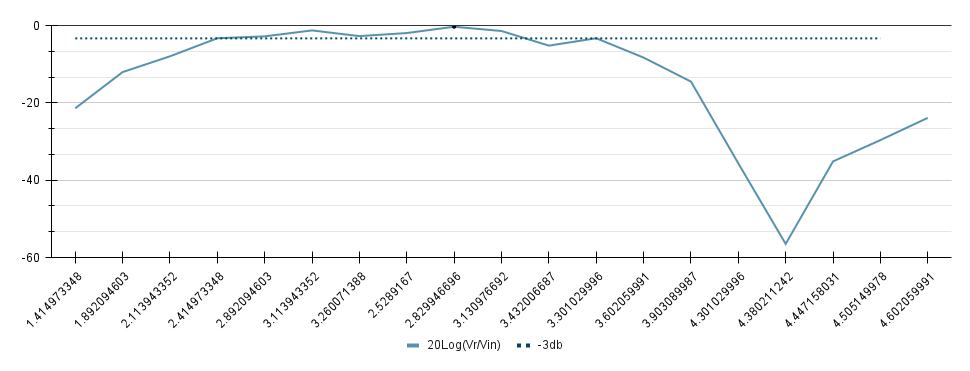
\includegraphics[width=0.7\textwidth]{assets/ch2.png}
    \caption{$20\log{V_r\over V_i}\ vs\ \log f$}
\end{figure}

The  $20\log{V_r\over V_in}$ was plotted vs $log\ f$, from the plot, we concluded that it is a band-pass filter with the 3db value crossing 2-values, 2.4 and 3.28, and in frequency, they are represented as $f_{c1} = 251.18Hz,\ f_{c2} = 1905.1Hz$  which are accepted values considering the theoretical and practical values.
\begin{figure}[H]
    \centering
    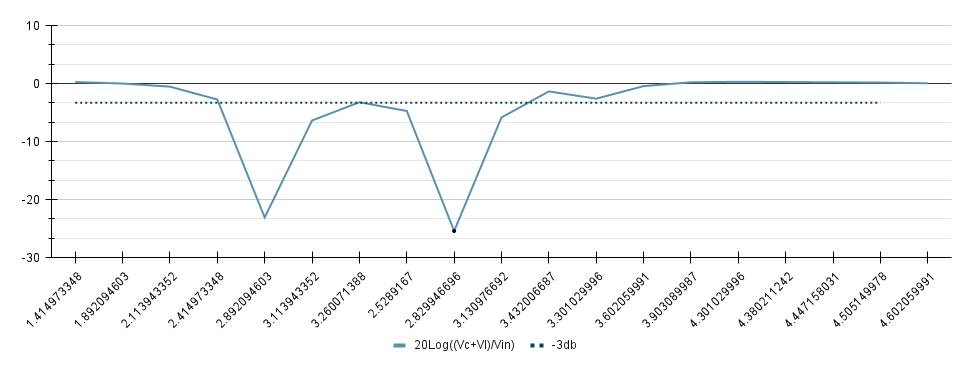
\includegraphics[width=0.7\textwidth]{assets/ch1.png}
    \caption{$20\log{V_c + V_L\over V_i}\ vs\ \log f$}
\end{figure}
We noticed, from the above graph, that $V_c + V_l$ has the same cut-off frequency as $V_r$ that we discussed earlier, and we notice that it is a band-reject filter but it has some error in the data so the values are caved in instated of going down as it should in the middle.
\hh{Active Filters}
\begin{figure}[H]
    \centering
    \begin{circuitikz}
        \ctikzset{bipoles/length=1cm}
        \draw
        (0, 0) node[op amp=$UA741$] (opamp) {}
        (opamp.-) to[R,l_=$1k\Omega$,-o] (-3, 0.35) 
        (opamp.-) to[short,*-] ++(0,0.5) coordinate (leftC)
        to[R=$2.2 k\Omega$] (leftC -| opamp.out)
        (opamp.-) to[short,*-] ++(0,1.5) coordinate (leftC) to[C=$220nF$] (leftC -| opamp.out) 
        to[short,-*] (opamp.out) to [short,-o] (2.5,0)
        (opamp.+) -- (-1,-0.35) to (-1,-0.75) node[ground]{}
        ;
        \node[font=\small] at (3, 0) {$V_o$};
        \node[font=\small] at (-4, 0.35) {$V_i$};
        \node[font=\small] at (0, -1) {UA741};
    \end{circuitikz}
    \caption{Active Low-Pass Filter}
\end{figure}
The circuit above was connected to $V_i$ with 2 Vrms amplitude and a cut-off frequency of $f_c$. We obtained $f_c$ using the same method used in (Figure \ref{meow-meow-n}) and we found it to have the value of 325.9 as shown in the following figure:
\begin{figure}[H]
    \centering
    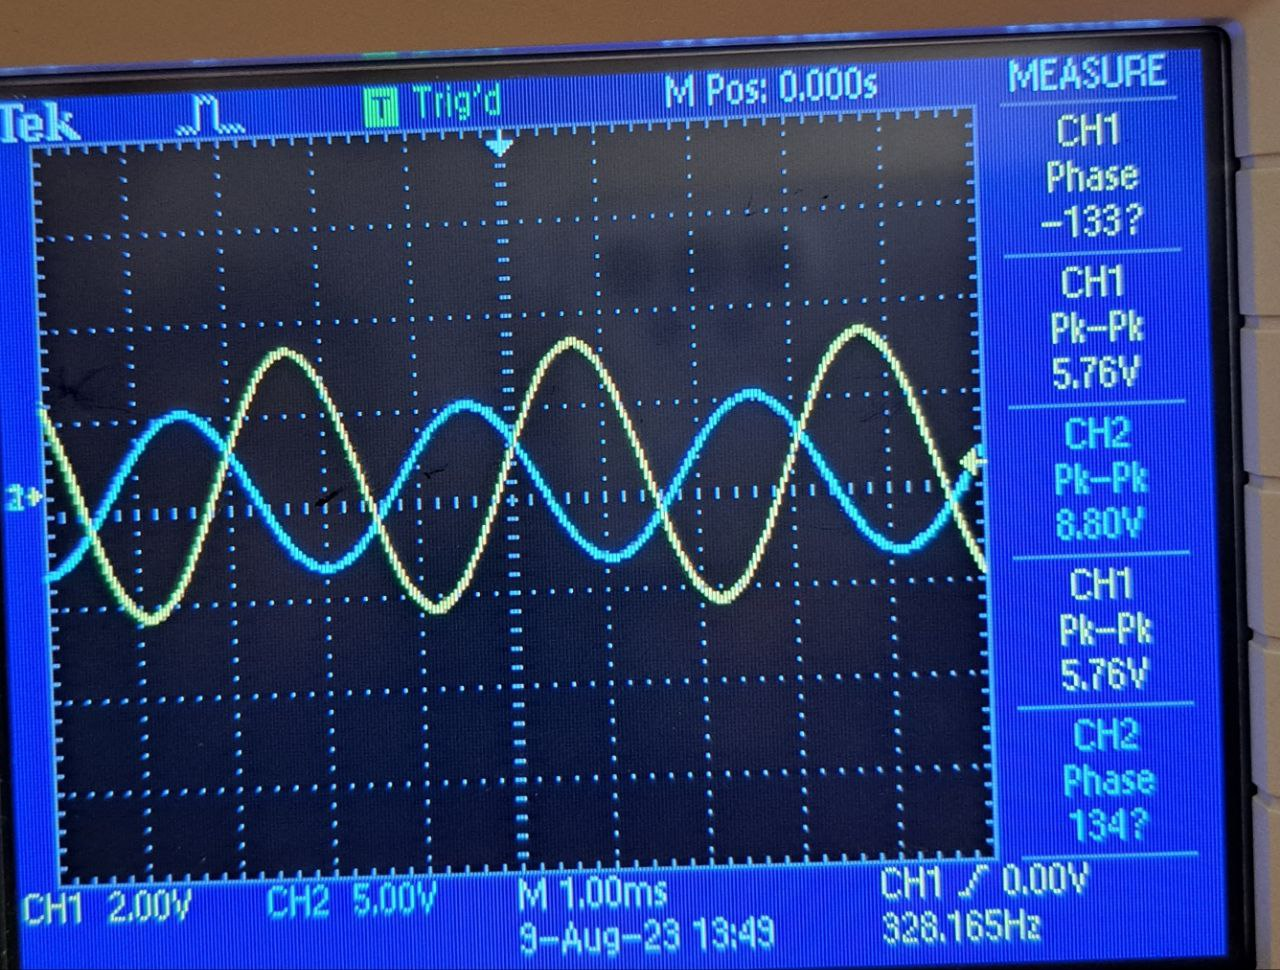
\includegraphics[width=0.5\textwidth]{assets/unnamed.jpg}
    \caption{Cut-off Frequency of the Active Low-pass filter}
\end{figure}
% Please add the following required packages to your document preamble:
% \usepackage{graphicx}
\begin{table}[H]
    \centering
    \resizebox{0.9\textwidth}{!}{%
    \begin{tabular}{|r|r|r|r|r|}
    \hline
    \multicolumn{1}{|l|}{Frequency} & \multicolumn{1}{l|}{Vin (Vrms)} & \multicolumn{1}{l|}{Vd (Vrms)} & \multicolumn{1}{l|}{log f} & \multicolumn{1}{l|}{20 log (Vd/Vin)} \\ \hline
    32.84  & 2 & 4.24 & 1.516403148 & 6.526717219   \\ \hline
    65.68  & 2 & 4.18 & 1.817433144 & 6.402925722   \\ \hline
    131.36 & 2 & 3.95 & 2.11846314  & 5.911341999   \\ \hline
    262.72 & 2 & 3.31 & 2.419493135 & 4.375959962   \\ \hline
    328.4  & 2 & 3    & 2.516403148 & 3.521825181   \\ \hline
    492.6  & 2 & 2.32 & 2.692494408 & 1.289159785   \\ \hline
    656.8  & 2 & 1.9  & 2.817433144 & -0.4455278942 \\ \hline
    1313.6 & 2 & 1.02 & 3.11846314  & -5.848596478  \\ \hline
    1970.4 & 2 & 0.69 & 3.294554399 & -9.243618099  \\ \hline
    3284   & 2 & 0.42 & 3.516403148 & -13.55561411  \\ \hline
    3940.8 & 2 & 0.35 & 3.595584394 & -15.13923903  \\ \hline
    6568   & 2 & 0.21 & 3.817433144 & -19.57621402  \\ \hline
    \end{tabular}%
    }
    \caption{High-pass filter data points}
    \label{tab:my-table}
    \end{table}
\begin{figure}[H]
    \centering
    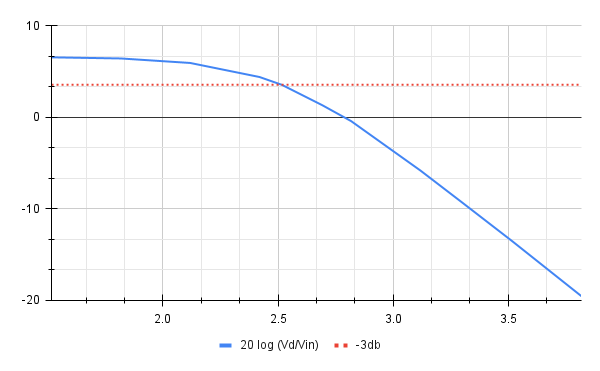
\includegraphics[width=0.6\textwidth]{assets/ch4.png}
    \caption{$20\log(Vd/Vi)$ over $log\ f$}
\end{figure}
From the above graph, we noticed that the low-pass filter has a cut-off frequency of $316.23 Hz$ which is an acceptable result since the theoretical value is $f_c = {1 \over 2\pi RC} = 328.83 Hz$.
\begin{figure}[H]
    \centering
    \resizebox{0.49\textwidth}{!}{
    \centering
    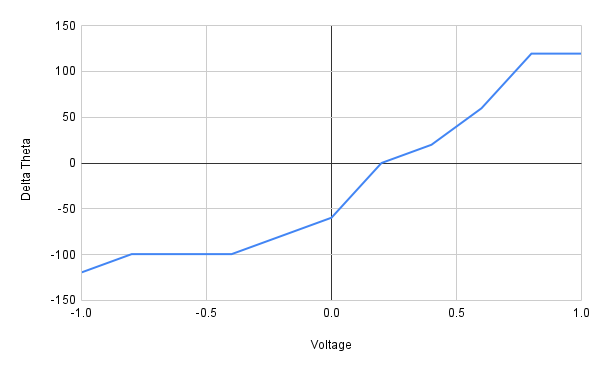
\includegraphics{assets/ch.png}
    }
    \resizebox{0.49\textwidth}{!}{
    \centering
    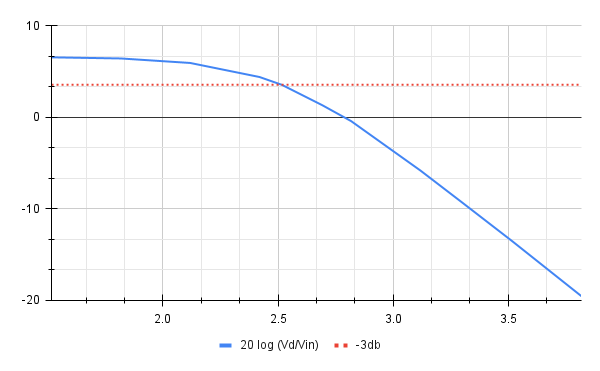
\includegraphics{assets/ch4.png}
    }
    \caption{Passive vs Active Low-pass filter}
\end{figure}
In comparison with the low-pass filter that we discussed (Figure: \ref{meow-meow-n}) we notice that the active filter is working as an amplifier with a maximum gain of $\approx 7dB$ while the passive filter is losing the amplitude with a gain under zero.
\clearpage
\h{Conclusion}
In conclusion, active filters are more efficient and have a higher gain than passive filters, filters work by attenuating the amplitude relative to unwanted frequency, and how the filter elements affect the input-to-output phase.
\clearpage
\bibliographystyle{plain}
\bibliography{cites}
\h*{Appendix}

\begin{figure}[H]
    \centering
    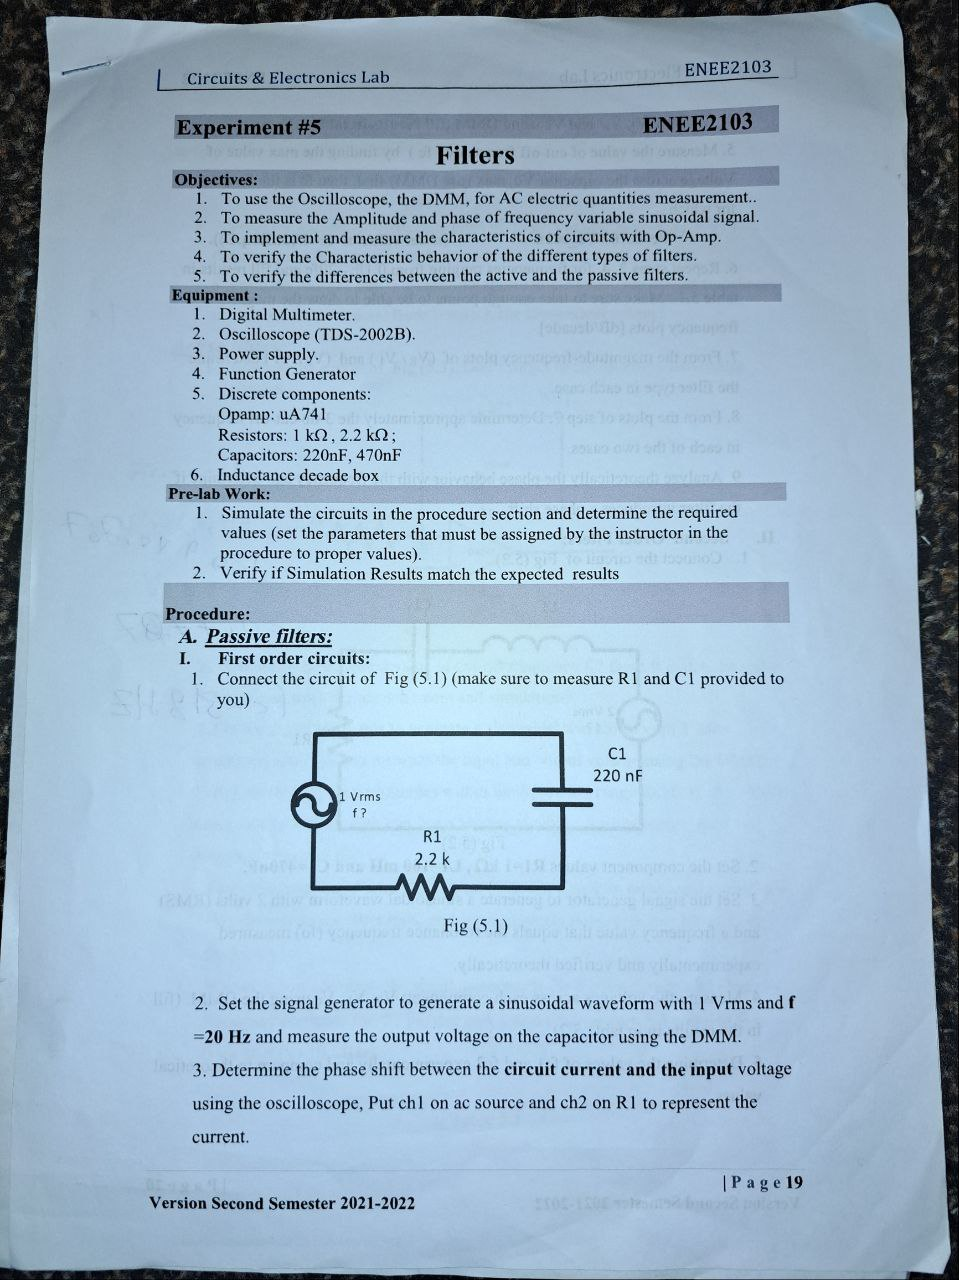
\includegraphics[width=\textwidth]{assets/i1.jpg}
    \caption{Page 1}
\end{figure}

\begin{figure}[H]
    \centering
    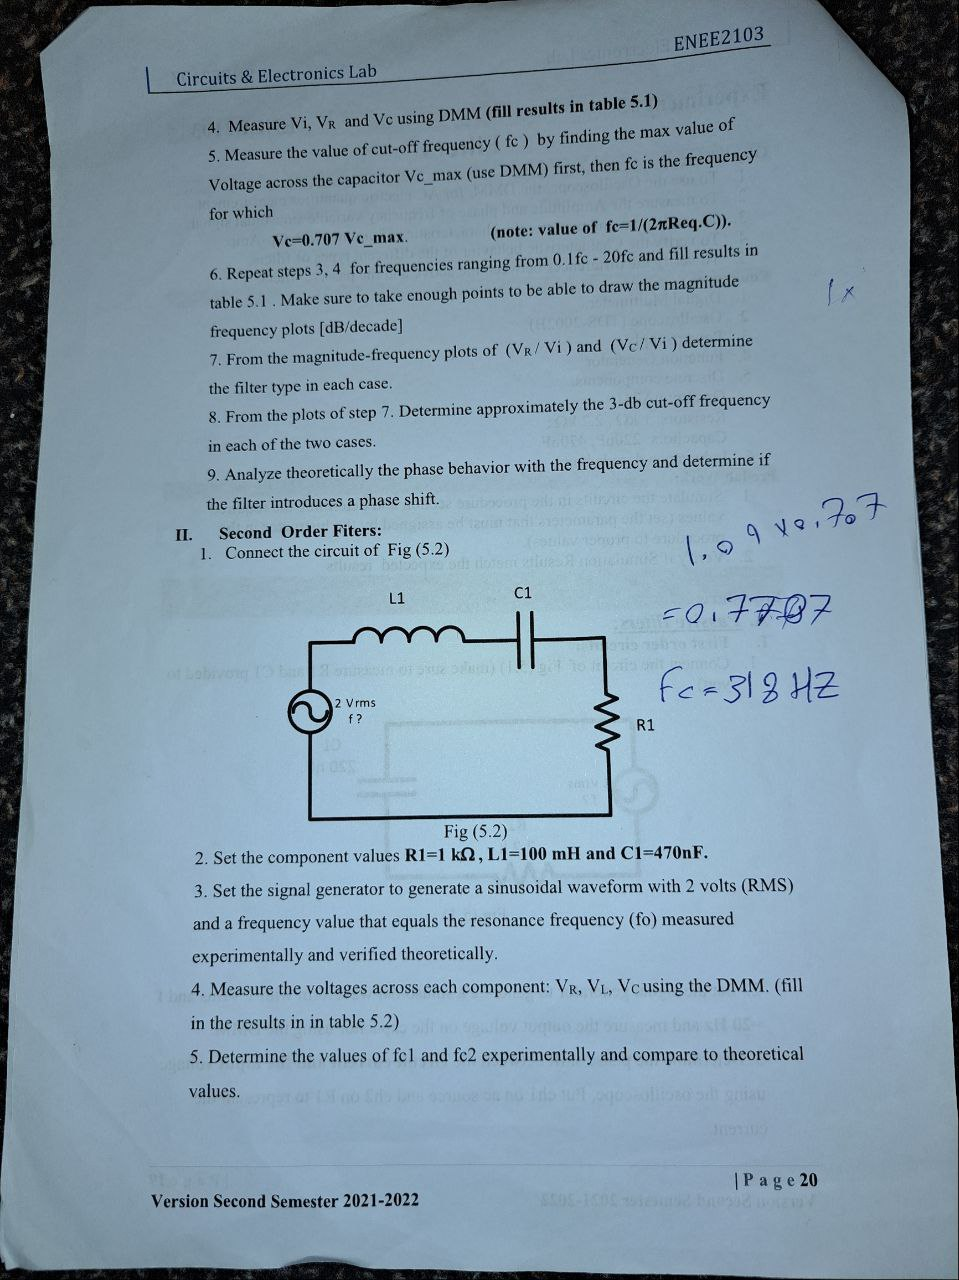
\includegraphics[width=\textwidth]{assets/i2.jpg}
    \caption{Page 2}
\end{figure}

\begin{figure}[H]
    \centering
    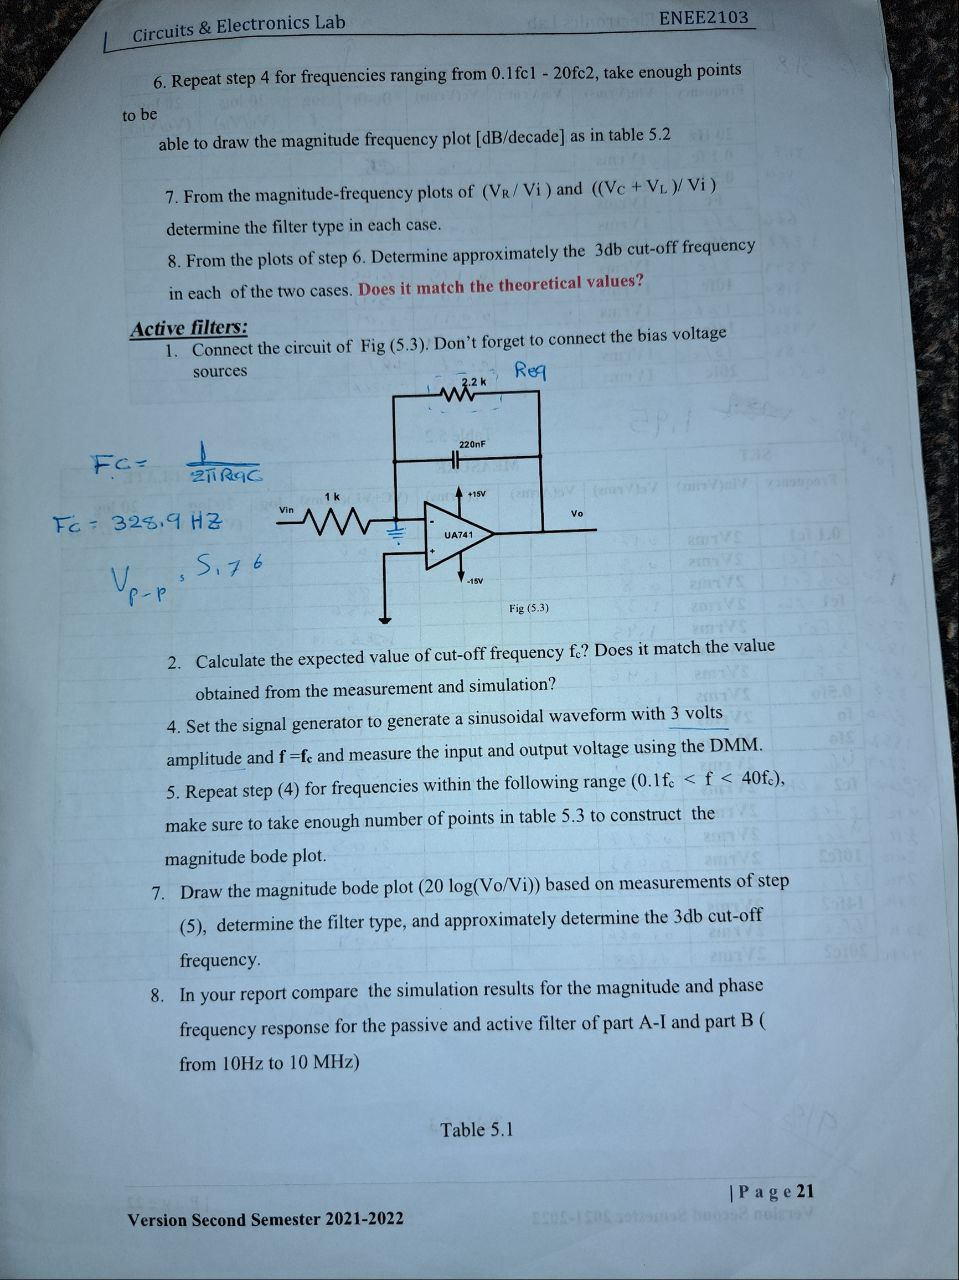
\includegraphics[width=\textwidth]{assets/i3.jpg}
    \caption{Page 3}
\end{figure}

\begin{figure}[H]
    \centering
    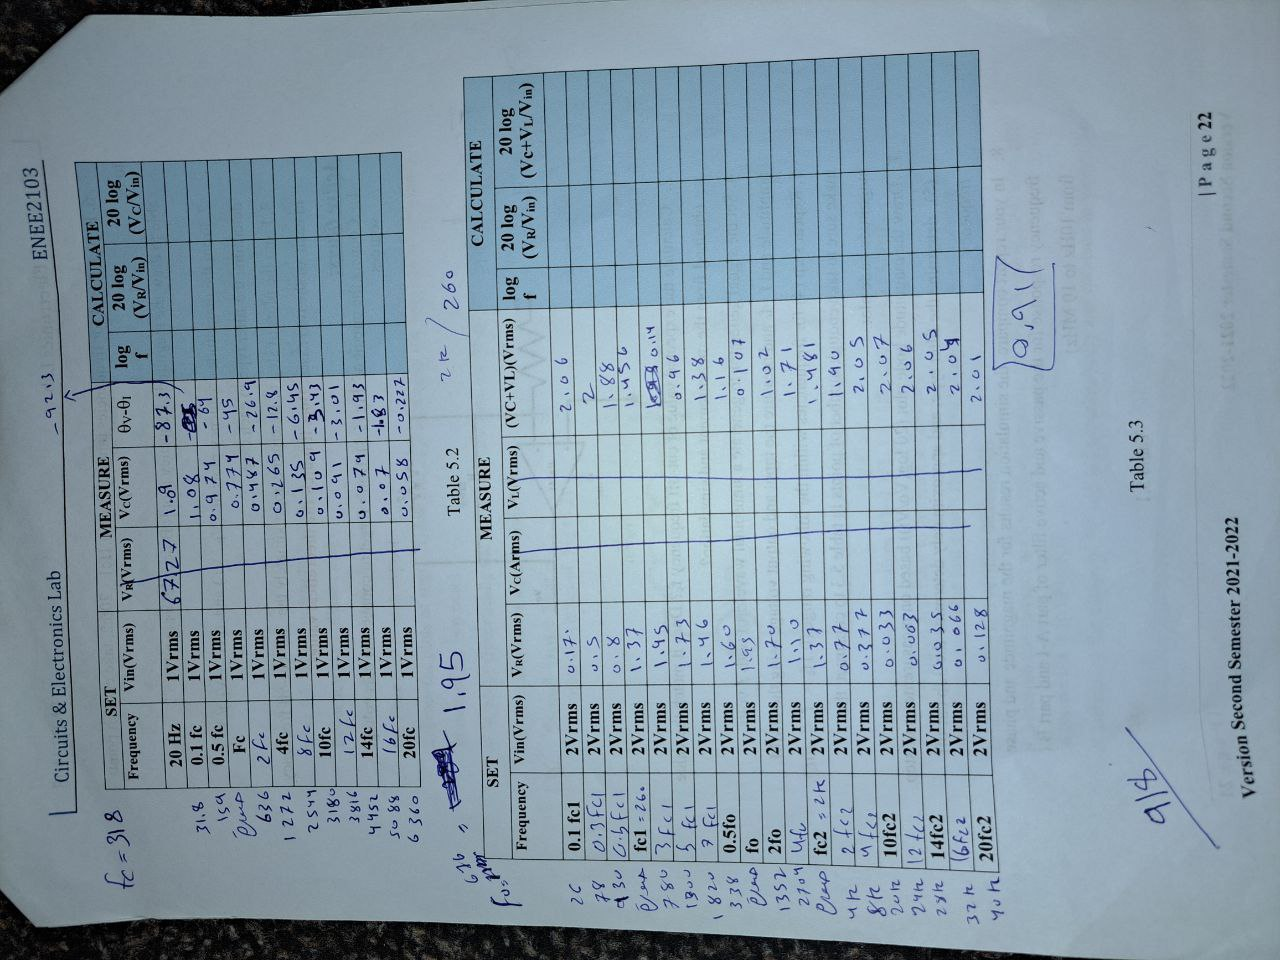
\includegraphics[width=\textwidth, angle=270]{assets/i4.jpg}
    \caption{Appendix - Page 4}
\end{figure}

\begin{figure}[H]
    \centering
    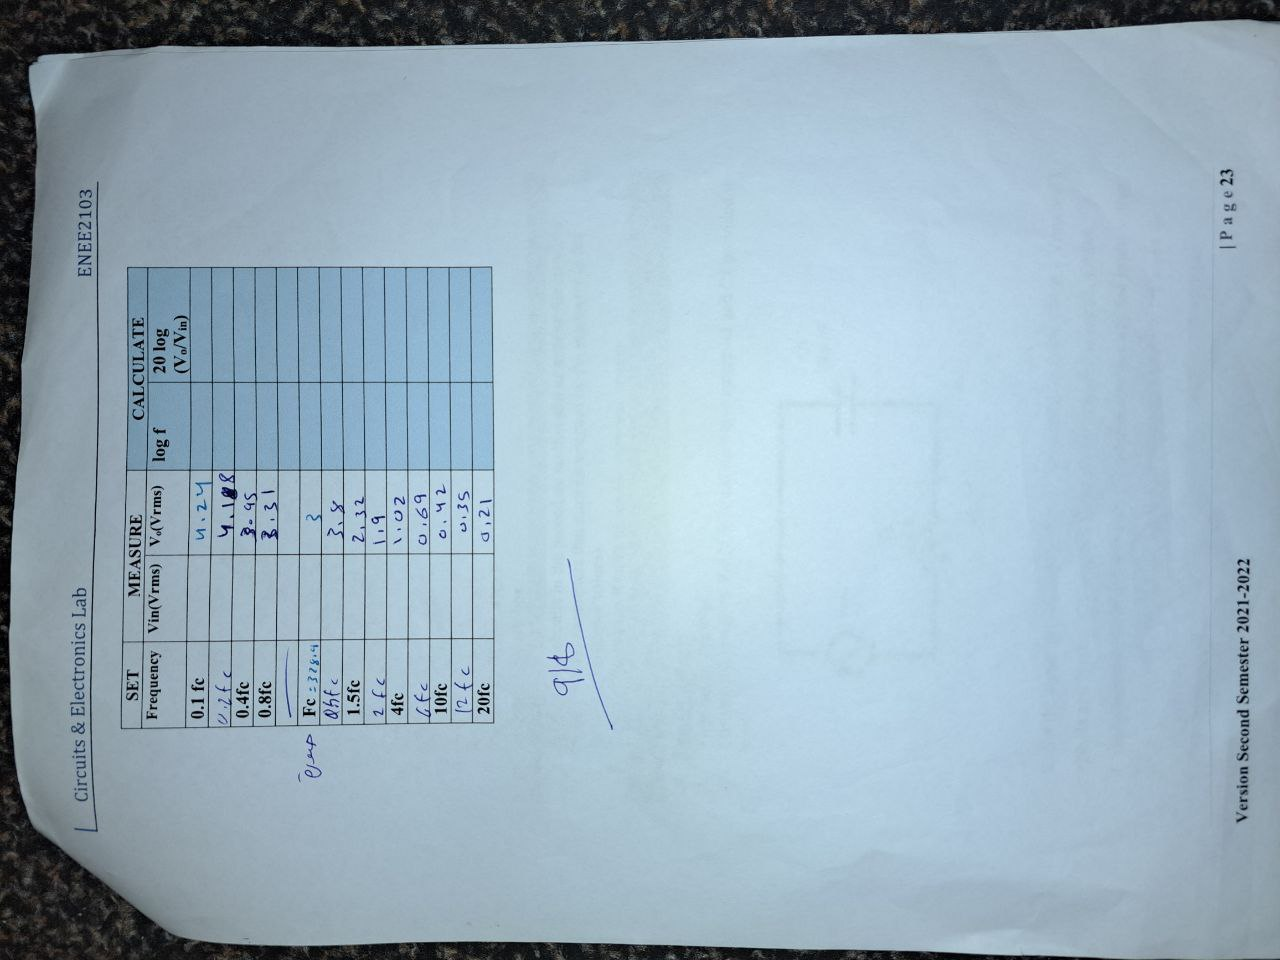
\includegraphics[width=\textwidth, angle=270]{assets/i5.jpg}
    \caption{Appendix - Appendix - Page 5}
\end{figure}

\end{document}




